%auto-ignore


\chapter{The Fatgraph Complex}
\label{cha:ribbon-graph-complex}

In \cite{kontsevich;1993} and \cite{kontsevich;feynman}, M. Kontsevich
introduced ``Graph Homology'' complexes that relate the stable
homology groups of certain infinite-dimensional Lie algebras to
various other topological objects, depending on the choice of an
operad.  In particular, the ``associative operad'' variant of the
construction gives birth to a chain complex whose homology is
isomorphic to the (co)homology of the moduli space of smooth punctured
curves $\M_{g,n}$.

Here we give a construction of the fatgraph complex, deriving it
as a relative of Thurston-Harer's arc-system complex \cite{%
  harer;cohomological-dimension,%
  harer;cohomology-of-moduli%
},\FIXME{%
  Rivedere attribuzione degli arc-system.}
and prove the isomorphism of its homology with the
rational (co)homology of $\M_{g,n}$.  The main ingredient of this
construction is a cell decomposition of $\M_{g,n}$ based on a theorem
of Jenkins and Strebel \cite{strebel;quadratic-differentials;1983}.
This ribbon graph complex is the same complex that one gets by
applying Kontsevich' construction in the associative case; however,
the proof given here is specific to $\M_{g,n}$ and does not trivially
extend to other cases.  The route to it is a bit convoluted, as the
direct approach to constructing a fatgraph complex by defining
face operators through contraction of edges does not yield a
simplicial complex: after a few contractions, loops appear, which
cannot be contracted any more.  This mirrors the structure of Harer's
$X - X_\infty$, as will be shown in Section~\ref{sec:cell-structure}.

In contrast to the simpler method presented here, the techniques
devised by Kontsevich are suitable to further generalization to any
``modular operad'' \cite{getzler-kapranov}.  A construction of the
graph complex, closely following Kontsevich' original work, has been
detailed in \cite{conant-vogtmann;2003}. Recently, Hamilton and
Lazarev gave a new proof in \cite{hamilton-lazarev;math.QA/0608395}.




\section{Moduli Spaces of Curves}
\label{sec:moduli-spaces}

Let us recap the main points of the construction of the moduli space
of smooth algebraic curves; the short summary given here tracks
closely the first section of \cite{looijenga;cellular-decomposition},
which has proofs and references.

Fix integers $g,n\geq0$ such that $2 -2g - n < 0$. Let $S$ be a Riemann
surface of genus $g$ and $P = \{ x_1, \ldots, x_n \}$ a set of $n$ points
in $S$.  

Let $\Diff(S,P)$ be the group of diffeomorphims of $S$ that fix $P$
pointwise; let $\Diff^0(S,P)$, resp.~$\Diff^+(S,P)$, be the subgroups
of diffeomorphisms homotopic to the identity mapping $\id_S$,
resp.~the subgroup of orientation-preserving diffeomorphisms.

Every set $P$ of marked points can be transformed into another chosen
set $P'$ (of the same cardinality) by a diffeomorphism $\phi$
homotopic to the identity mapping $\id_S$.  Therefore, $\Diff^+(S,P)$
and $\Diff^0(S, P)$ depend only on $n = \card{P}$ and not on $P$,
cf. \cite{krushkal;riemann-surfaces}.  Summing up:
\begin{definition}\label{dfn:diff}
  $\Diff(S,n)$ is the group of orientation-preserving diffeomorphisms
  that keep the $n$ marked points fixed.

  $\Diff^0(S,n)$ is the group of diffeomorphisms of $S$ which are
  homotopic to the identity mapping $\id_S$ and that keep the $n$
  marked points fixed.
\end{definition}

Every complex structure  on $S$ determines a conformal structure; let
$\Conf(S)$ be the set of all conformal structures on $S$. 
\begin{definition}\label{dfn:teichmuller}
  The Teichm{\"u}ller space
  \begin{equation*}
    \T_{g,n} := \Conf(S) / \Diff^0(S, n)
  \end{equation*}
  is the quotient of the set of all conformal metrics on $S$ by the
  set of all diffeomorphisms homotopic to the identity and fixing the
  $n$ marked points.
\end{definition}
The Teichm{\"u}ller space $\T_{g,n}$ is an analytic space and is
homeomorphic to a convex domain in $\setC^{3g - 3 + n}$.

\begin{definition}\label{dfn:mapping-class-group}
  The mapping class group $\Gamma_{g,n}$ is the set of connected components
  of $\Diff^+(S, n)$, the group of all diffeomorphisms that preserve
  orientation and fix marked points:
  \begin{equation*}
    \Gamma_{g,n} := \Diff^+ (S, n) / \Diff^0(S, n).
  \end{equation*}
\end{definition}


\subsection{Moduli space of smooth curves}
\label{sec:Mgn}

\begin{definition}
  The topological space $\M_{g,n} := \T_{g,n} / \Gamma_{g,n}$ is the
  moduli space of (smooth) $n$-pointed algebraic curves of genus $g$.
  It parametrizes complex structures on $S$, up to
  diffeomorphisms that:
  \begin{inparaenum}
  \item are homotopic to the identity mapping on $S$,
  \item preserve the orientation of $S$, and
  \item fix the $n$ marked points.
  \end{inparaenum}
\end{definition}
Since $\T_{g,n}$ is an analytic variety and $\Gamma_{g,n}$ acts
discontinuously with finite stabilizers, $\M_{g,n}$ inherits a
structure of analytic orbifold of complex dimension $3g - 3 + n$.

Since $\T_{g,n}$ is contractible, its equivariant (co)homology with
rational coefficients is isomorphic to the rational (co)homology of
$\M_{g,n}$ (see \cite[VII.7.7]{brown}):
\begin{equation}
  \label{eq:rational-homology-of-Mgn-from-equivariant-homology-of-Tgn}
  H^{\Gamma_{g,n}}_*(\T_{g,n}, \setQ) \cong H_*(\M_{g,n}, \setQ),
  \qquad
  H_{\Gamma_{g,n}}^*(\T_{g,n}, \setQ) \cong H^*(\M_{g,n}, \setQ),
\end{equation}

\subsubsection{Alternate descriptions of $\M_{g,n}$}
\label{sec:alternate-Mgn}
One may instead consider equivalence classes of $n$-punctured surfaces
$S$ (i.e., with $n$ points \emph{removed}) by bianalytic mappings that
do \emph{not} permute the punctures, and repeat the same construction
of the Teichm\"uller and the moduli space.  By the Riemann extension
theorem, the two approaches turn out to yield the same result.

Another approach leads to the construction of $\M_{g,n}$ by
equivalence classes of triples $(C, x, f)$ where $C$ is a complex
curve, $x: \{1, \ldots, n\} \longrightarrow C$ a marking of points,
and $f: C \to S$ a homeomorphism with a fixed reference topological
Riemann surface $S$.

In the course of this chapter, we will make use of the description of
$\M_{g,n}$ that best fits in the context, often without explicit
notice.  In particular, we shall consider points $x_1$, \ldots, $x_n$ as
marked points or as punctures, interchangeably.

\subsection{Moduli Space of stable curves}
\label{sec:moduli-space-stable}

Deligne and Mumford \cite{deligne-mumford} showed that $\M_{g,n}$ has
a projective compactification $\Mbar_{g,n}$; this space can be
described as the moduli space of stable curves of arithmetic genus
$g$.
\begin{definition}
  A stable complex curve $C$ is a complete connected curve such that:
  \begin{enumerate}
  \item $C$ has only nodal singularities;
  \item the marked points $x_1, \ldots, x_n$ are nonsingular points in
    $C$;
  \item the pair $(C; x_1, \ldots, x_n)$ has a \emph{finite} automorphism
    group.
  \end{enumerate}
\end{definition}
Equivalently, this last condition can be expressed by saying that:
\begin{inparaenum}[\slshape a)]
\item any rational component of the normalized curve $\tilde C$
  must contain at least 3 special points --- i.e., marked points or
  singular points;
\item  any component of genus $1$ must contain
  at least 1 special point.
\end{inparaenum}

Let $C$ be a stable curve, with $\nu$ irreducible components and $r$
nodal points. Let $\{C_j\}_{j=1, \dots, \nu}$ be the irreducible
components of $C$ and $g(C_j)$ the geometric genus of $C_j$.  The
arithmetic genus of $C$ is defined by the equation:
\begin{equation*}
  p(C) := \bigl({\textstyle \sum_{j=1}^\nu} g(C_j) \bigr) + r - \nu + 1.
\end{equation*}

Informally, stable curves are constructed by attaching smooth curves
``by the nodes'', such that the arithmetic genus be $g$ and the total
number of punctures be $n$.



\section{Fatgraphs}
\label{sec:fatgraphs}

``Fatgraphs'' take their name from being usually depicted as graphs
with thin bands as edges, instead of 1-dimensional lines; they have
also been called ``Ribbon graphs'' in the literature.  The two names
will be used interchangeably here.

\begin{definition}
  \label{dfn:fatgraphs}
  A fatgraph is a finite CW-complex of pure dimension 1, together
  with an assignment, for each vertex $\gamma$, of a cyclic ordering of the
  edges incident at $\gamma$.

  A morphism of fatgraphs is a cellular map $f:G\to G'$ such that,
  for each vertex $\gamma$ of $G'$, the preimage $f^{-1}(V)$ of a small
  neighbourhood $V$ of $\gamma$ is a small neighbourhood of a tree in $G$
  (i.e., it is a connected graph with no nontrivial homological
  cycles).
\end{definition}
Unless otherwise specified, we assume that all vertices of a ribbon
graph have valence at least 3.

If $G$ is a fatgraph, denote $\Vertices{G}$, $\Edges{G}$ and
$\Legs{G}$ the sets of vertices, unoriented edges and oriented edges
(at times called ``legs'' or ``half-edges'').

\subsubsection{Morphisms arising from contraction of an edge}
\label{sec:contractions}
Let $G$ be a fatgraph, and $G'$ be the CW-complex obtained by
contracting an edge $\alpha \in \Edges{G}$ to a point.  If $\alpha$ connects two
\emph{distinct} vertices, that is, $\alpha$ is not a loop, then $G'$
inherits a fatgraph structure from $G$: if $(\alpha < \alpha_1 < \ldots < \alpha_k <
\alpha)$ and $(\alpha < \alpha'_1 < ... < \alpha'_h < \alpha)$ are the cyclic orders at
endpoints of $\alpha$, then the vertex formed by collapsing $\alpha$ is endowed
with the cyclic order $(\alpha_1 < \ldots < \alpha_k < \alpha'_1 < \ldots < \alpha'_h)$.  The
contraction morphisms play a major role in manipulation of ribbon
graphs.

The following lemma is an immediate consequence of the definition.
\begin{lemma}\label{lemma:contraction1}
  Any morphism of fatgraphs is a composition of isomorphisms and
  contractions of non-loop edges.
\end{lemma}

We can thus define functors $\Vertices{-}$, $\Edges{-}$ and $\Legs{-}$
that take a morphism of graphs to a map of their set of vertices,
(unoriented) edges, and oriented edges.

\subsection{From fatgraphs to Riemann surfaces, I}
\label{sec:rg-to-surfaces}

There is a functorial construction to build a topological surface
$S(G)$ from a fatgraph $G$; this is usually referred to as
``thickening'' or ``fattening'' in the literature.

\begin{lemma}
  A fatgraph is uniquely determined by the following data: a
  finite set $L$ together with bijective maps $\sigma_0, \sigma_1, \sigma_2: L \to L$ such
  that:
  \begin{itemize}
  \item $\sigma_1$ is involutive: $\sigma_1^2 = \id$, and
  \item $\sigma_0 \circ \sigma_2 = \sigma_1$.
  \end{itemize}
\end{lemma}
\begin{proof}
  To pass from the topological description to the combinatorial one,
  take $L$ to be the set of \emph{oriented} edges of the CW-complex
  underlying a fatgraph.  Define $\sigma_1:L\to L$ as the orientation
  reversal on edges.  Define $\sigma_0:L\to L$ by means of the cyclic order
  at vertices: let $L(\gamma)$ be the subset of edges in $L$ that
  \emph{end} at a vertex $\gamma$, the cyclic order on edges incident at
  $\gamma$ induces a cyclic order on $L(\gamma)$.  If $l\in L(\gamma)$ then
  define $\sigma_0(l)$ as the successor to $l$ in the cyclic order on
  $L(\gamma)$.  Finally, define $\sigma_2: L \to L$ by means of
  $\sigma_2=\sigma_0^{-1}\sigma_1$.

  Vice versa, let $L_i$ be the set of orbits of the map $\sigma_i$.  Take
  $L_0$ to be the set of 0-cells; for each $\{l,l'\} \in L_1$, glue a
  1-cell to the 0-cells corresponding to the $\sigma_0$-orbits of $l$ and
  $l'$.  The cyclic order at each vertex is induced by the action of
  $\sigma_0$.
\end{proof}
Any two of the maps $\sigma_0, \sigma_1, \sigma_2$ determine the third, by means of
the defining relation $\sigma_0 \circ \sigma_2 = \sigma_1$; therefore, to give a ribbon
graph, it is sufficient to specify only two out of three maps.

In the combinatorial description, $\Vertices{G}$ is the set $L_0$ of
orbits of $\sigma_0$, $\Edges{G}$ is the set $L_1$ of orbits of $\sigma_1$, and
$\Legs{G}$ is plainly the set $L$.  

\begin{lemma}
  \label{lemma:S-functor}
  \begin{inparaenum}
  \item There is a functor $S$ that associates to every fatgraph
    $G$ a punctured Riemann surface $S(G)$, and to every morphism $f:
    G \to G'$ a continuous map $S(f): S(G) \to S(G')$.
  \item The surface $S(G)$ is naturally endowed with a triangulation
    indexed by oriented edges of $G$.
  \end{inparaenum}
\end{lemma}
\begin{proof}
  Let $G = (L; \sigma_0, \sigma_1, \sigma_2)$ be a fatgraph.  Pick a
  topological 0-cell for each $\sigma_0$-orbit in $L$, and a 1-cell
  for each $\sigma_1$-orbit; attach the 1-cell $\alpha = \{\alpha^+,
  \alpha^-\}$ to the (possibly not distinct) 0-cells corresponding to
  the $\sigma_0$-orbits of $\alpha^+$ and $\alpha^-$.  Now glue a
  punctured 2-cell $B_\beta^\times$ along any $\sigma_2$-orbit
  $\beta$: if $\{l, \sigma_2(l), \ldots, \sigma_2^k(l)\}$ is a
  $\sigma_2$-orbit (in the order it is swept by $\sigma_2$) and
  $\sigma_2^{k+1}(l) = l$, then attach a punctured 2-disk so that its
  oriented border is the 1-cycle formed by the graph edges
  corresponding to $\sigma_2^i(l)$.

  To describe the triangulation of $S(G)$, assume at first that $G$
  has no loops.  In the course of the construction of $S(G)$, a
  punctured disk $B_\beta^\times$ has been glued to each
  $\sigma_2$-orbit $\beta$; for each oriented edge $\alpha^\pm \in
  \beta$, let $T_{\alpha^\pm}^{(\beta)}$ be the curvilinear triangle
  delimited by $\alpha^\pm$ and the radii joining endpoints of
  $\alpha^\pm$ with the center of $B_\beta$.  The collection $\{
  T_{\alpha^\pm}^{(\beta)} \}$ is a triangulation of $S(G)$.  When $G$
  has a loop $\alpha$, there is a $\sigma_2$-orbit $\beta$ such that
  $\beta$ is made of an oriented edge $\alpha^\pm \in \alpha$ alone,
  thus $B_\beta$ is bounded by $\alpha^\pm$ only.  Split $\alpha^\pm$
  at the midpoint to form two edges $\alpha'$, $\alpha''$: then
  $B_\beta$ breaks up into triangles $T_{\alpha'}$ and $T_{\alpha''}$
  and we can proceed as before.

  Finally, for every morphism $f: G \to G'$ build a continuous map
  $S(f): S(G) \to S(G')$ by mapping $T_\alpha$ homeomorphically onto $T_{\alpha'}$
  if $f$ maps $\alpha$ onto $\alpha'$, or contracting $T_\alpha^{(\beta)}$ to a radius of
  $B_\beta$ if $f$ contracts $\alpha$ to a point.
\end{proof}
Thus we have constructed a punctured Riemann surface $S(G)$, such that
$G$ is a deformation retract of $S(G)$.  Denote by $\Holes{G}$ the set
$L_2$ of orbits of $\sigma_2$; in the topological descpription, its
elements are the support of 1-cycles in $H^1(G)$ that correspond under
the retraction to small loops around the punctures in $S(G)$; they are
called ``boundary components'' of $G$.  Also in the topological
description, it will be convenient to identify a boundary component
$\beta$ with the set of edges it is made of, and a vertex $\gamma$ with the set
of edges incident to it.  

The assignment $G \mapsto \Holes{G}$ extends to a functor $\Holes{-}$;
by Lemma~\ref{lemma:contraction1}, for any $f\colon G_1 \to G_2$ the
map $\Holes{f} \colon \Holes{G_1} \to \Holes{G_2}$ is a bijection.

\subsection{Numbered fatgraphs}
\label{sec:numbered-rg}

\begin{definition}
  A \emph{numbered fatgraph} is a fatgraph $G$ endowed with a
  bijection $\nu: \Holes{G} \to \{1,\ldots, n\}$.  The map $\nu$ is
  said to be a ``numbering'' on $G$.

  A morphism $f: G_1 \to G_2$ of numbered fatgraphs must preserve the
  numbering of boundary components:
  \begin{equation*}
    \xymatrix{%
      \Holes{G_1} &  & \Holes{G_2}
      \\
      & \{ 1, \ldots, n \} &
      \ar^{f} "1,1";"1,3"
      \ar_{\nu_1} "1,1";"2,2"
      \ar^{\nu_2} "1,3";"2,2"
    }%
  \end{equation*}
\end{definition}

Until the end of this chapter, \emph{all fatgraphs are implicitly
  equipped with a numbering}. By a slight abuse of language, we shall
usually omit mention of the numbering $\nu$ and just speak of ``the
numbered fatgraph $G$''.

The correspondence between fatgraphs and Riemann surfaces allows
us to give the following.
\begin{definition}\label{dfn:rg-genus}
  The \emph{puncture number} of a graph $G$ is given by $n =
  \card{\Holes{G}}$, and is equal to the puncture number of the
  Riemann surface $S(G)$.

  If $S(G)$ has genus $g$ and $n$ punctures, then:
  \begin{equation}
    \label{eq:euler-characteristics-of-fatgraphs}
    \chi(G) = \chi(S(G)) = 2 - 2g - n = 2 - 2g - \card{\Holes{G}},
  \end{equation}
  so we can define, for any fatgraph $G$, the \emph{genus} $g$, as
  given by the above relation.
\end{definition}
It is trivial to check the following.
\begin{lemma}\label{lemma:contraction2}
  If $G'$ is obtained from $G$ by contraction of a non-loop edge,
  then $G$ and $G'$ share the same genus and puncture number.
\end{lemma}
Denote by $\RG$ the category of numbered fatgraphs and their
morphisms.  By lemmas~\ref{lemma:contraction1}
and~\ref{lemma:contraction2}, $\RG$ decomposes into the disjoint union
of sub-categories $\RG_{g,n}$ whose objects are fatgraphs of genus
$g$ with $n$ punctures:
\begin{equation*}
  \RG = \coprod_{g,n} \RG_{g,n}
\end{equation*}
No morphism connects an object of $\RG_{g,n}$ with an object of
$\RG_{g',n'}$.


\subsection{Embedded fatgraphs}
\label{sec:embedded-rg}

Fix a reference Riemann surface $S = S_{g,n}$ of genus $g$ with $n$
punctures.

An embedding of a fatgraph $G$ is a injective continuous map $\iota:G\to
S$, that is, a homeomorphism of $G$ onto $\iota(G) \subseteq S$, such that the
orientation on $S$ induces the cyclic order at the vertices of $\iota(G)$.

When confusion is likely to arise, we shall speak of \emph{abstract}
fatgraphs, to mean the topological and combinatorial objects
defined in Definition~\ref{dfn:fatgraphs}, as opposed to \emph{embedded}
fatgraphs as in Definition~\ref{dfn:embedded-rg} below.

\begin{definition}\label{dfn:embedded-rg}
  An embedded fatgraph is a fatgraph $G$ endowed with a
  homeomorphism ${\tilde \iota}$ between $S(G)$ and the ambient
  surface $S$, modulo the action of $\Diff^0(S)$.
\end{definition}
Spelling out all details, an embedded fatgraph is an equivalence
class, modulo the action of $\Diff_0(S)$, of triples $[G, \iota,
\{\psi_i\}_{i=1}^n]$ composed of a numbered fatgraph $G$, an
embedding $\iota:G\to S$, and, for each connected component $C_i$ of
$S - \iota(G)$, a map $\psi_i: {\bar C_i} \to {\bar B}^\times$ such
that:
\begin{inparaenum}[\slshape (1)]
\item $\psi_i$ is a homeomorphism of the interior of $C_i$ with the
  punctured open unit disk $B^\times$;
\item $\psi_i$ restricts to $\iota^{-1}$ on the border $\partial C_i$.
\end{inparaenum}

Since a morphism $f:G\to G'$ of abstract fatgraphs induces a morphism
$S(f):S(G)\to S(G')$, then a morphism of embedded fatgraphs is
determined by a homotopy connecting ${\tilde \iota}$ and ${\tilde
  \iota' \circ f}$.  In detail: a morphism $[f]$ from $[G, \iota,
\psi_*]$ to $[G', \iota', \psi'_*]$ is given by the following data:
\begin{itemize}
\item an abstract fatgraph morphism $f:G\to G'$;
\item a homotopy $\eta:[0,1] \times S\to S$, such that:
  \begin{itemize}
  \item $\eta(0,-) = \id_S$,
  \item $\eta(1,-)$ transforms $\iota$ into $\iota' \circ f$
    and $\psi_i$ into $\psi'_i$.
  \end{itemize}

\end{itemize}

Embedded numbered fatgraphs with their morphisms form a category
$\ERG$, which is again the disjoint union of categories $\ERG_{g,n}$.
There is an obvious forgetful functor from the category of embedded
fatgraphs to the category of abstract numbered fatgraphs,
sending $[G, \iota] \mapsto G$ and $[f] \mapsto f$.

The mapping class group $\Gamma_{g,n}$ acts functorially on
$\ERG_{g,n}$ by changing the embedding: $\phi \in \Gamma_{g,n}$ maps
$[G, \iota, \psi_*]$ into $[G, \iota \circ \phi, \phi \circ \psi_*]$.

\begin{lemma}
  \label{lemma:erg-no-aut}
  An embedded fatgraph has no automorphisms other than the identity.
\end{lemma}
\begin{proof}
  Suppose $[f] \in \Aut_{\ERG}[G, \iota, \psi_*]$, then $f:G\to G$ is an abstract
  fatgraph automorphism, so it induces a $S(f): S(G) \to S(G)$
  which is a \emph{homeomorphism}.  By definition, there is a homotopy
  connecting ${\tilde \iota}: S(G) \to S$ and ${\tilde \iota'} \circ {\tilde f}:
  S(G)\to S$, so there is a homotopy connecting ${\tilde \iota'} \circ {\tilde f}
  \circ {\tilde \iota}^{-1}$ and $\id_S$, therefore $S(f)$ is a
  homeomorphism homotopic to the identity.  Thus, $\iota$ and $\iota'$ belong
  to the same class with respect to the action of $\Diff_0$, $[G, \iota,
  \psi_*] = [G, \iota', \psi'_*]$ and $[f]$ is the identity morphism.
\end{proof}


\subsection[From graphs to surfaces, II][A complex analytic atlas on $S(G)$]
{From graphs to surfaces, II: a complex analytic atlas on $S(G)$}
\label{sec:atlas}

We can give the topological Riemann surface $S(G)$ a complex analytic
structure by means of the triangulation in \ref{lemma:S-functor}(b)
and an analytic atlas.

Recall that in Lemma~\ref{lemma:S-functor}, a triangulation of the surface
$S(G)$ was defined, featuring a simplex $T_{\alpha^\pm}$ for each
non-loop oriented edge, and two distinct simplexes for each oriented
loop in $G$.

Define an atlas of $S(G)$:
\begin{itemize}
\item For any non-loop edge $\alpha \in \Edges{G}$, let $V_\alpha :=
  (T_\alpha^+ \cup T_\alpha^-)^\circ$ be the interior of the union of
  the two triangles having $\alpha$ as an edge.  Similarly, for each loop edge
  $\lambda$, construct domains $V_{\lambda'}$, $V_{\lambda''}$ from
  the two halves $\lambda'$, $\lambda''$ that $\lambda$ is cut into
  in the construction of Lemma~\ref{lemma:S-functor}.
\item For any boundary component $\beta \in \Holes{G}$, put $V_\beta := \bigl(
  \bigcup_{\alpha} T_\alpha^{(\beta)} \bigr)^\circ$, the interior part of the union of triangles
  bounded by all edges $\alpha$ bounding $\beta$.
\item For any vertex $\gamma \in \Vertices{G}$, put $V_\gamma := \bigl( \bigcup_\alpha T_a^\pm
  \bigr)^\circ$, the interior part of the union of triangles bounded by
  edges $\alpha$ incident to $\gamma$.
\end{itemize}
\begin{figure}[btp]
  %% Figura atlas.fig
  \centering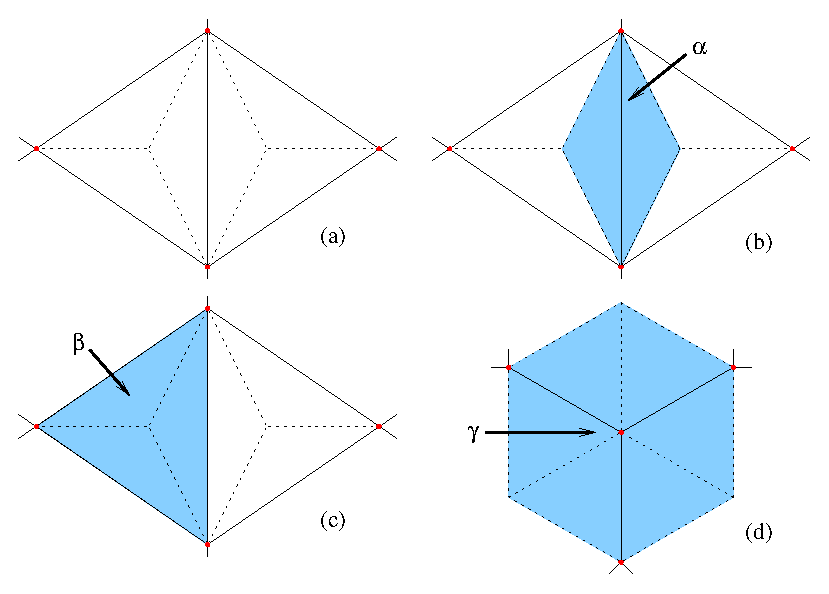
\includegraphics[width=\textwidth]{atlas}
  \caption{The open sets building an atlas of $S(G)$: \textsl{(a)} the
    triangulation built from a graph $G$: graph edges are drawn as
    solid lines, and edges of $T_\alpha^{\pm}$ are drawn as dotted
    lines; \textsl{(b)} the neighborhood $V_\alpha$ of an edge
    $\alpha$; \textsl{(c)} the neighborhood $V_\beta$ of a boundary
    component $\beta$; \textsl{(d)} the neighborhood $V_\gamma$ of a
    vertex $\gamma$.}
  \label{fig:atlas}
\end{figure}

\begin{definition}
  \label{dfn:metric-ribbon-graphs}
  A metric $\ell$ on a fatgraph $G$ is an assignment of a real
  positive number $\ell_\alpha$ for each edge $\alpha \in \Edges{G}$.

  A metrized fatgraph $(G, \ell)$ is a fatgraph $G$ equipped with
  a metric $\ell$.
\end{definition}

Given a metric $\ell$ on the graph $G$, define charts on the open sets
$V_*$ (see Figure~\ref{fig:charts}):
\begin{itemize}
\item for any non-loop edge $\alpha$, pick a homeomorphism $f_\alpha: V_\alpha \to \{ z \in \setC
  : 0 < \Re z < \ell_\alpha \}$; for any loop $\lambda$, choose
  homeomorphisms $f_{\lambda'}, f_{\lambda''}: V_{\lambda'}, V_{\lambda''} \to \{ z \in \setC
  : 0 < \Re z < 1/2 \cdot \ell_\alpha \}$;
\item for any boundary component $\beta$, bounded by edges $\alpha_1$, $\alpha_2$
  and $\alpha_3$, pick a homeomorphism $f_\beta: V_\beta \to \{ \abs{z} < \rho \}$, where
  $\rho = (\ell_{\alpha_1} + \ell_{\alpha_2} + \ell_{\alpha_3}) / 2\pi$.
\item for any vertex $\gamma$, pick a homeomorphism $f_\gamma: V_\gamma \to \setC$.
\end{itemize}
\begin{figure}[htbp]
  %% Figura charts.fig
  \centering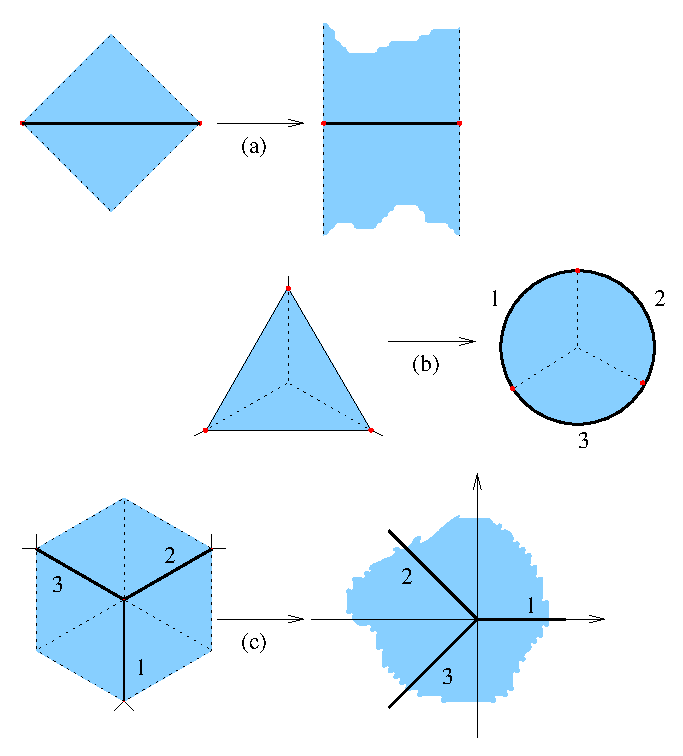
\includegraphics{charts}
  \caption{Local charts on the atlas: \textsl{(a)} any open set
    $V_\alpha$ maps to a strip in the complex plane; \textsl{(b)} any
    open set $V_\beta$ maps to a disk; \textsl{(c)} any open set
    $V_\gamma$ maps to the complex plane itself.}
  \label{fig:charts}
\end{figure}
These choices are subject to the condition that transition functions
satisfy the following:
\begin{itemize}
\item if $\alpha$ is an edge bounding the boundary component $\beta$, then $f_\beta
  \circ f_\alpha^{-1} = \exp (2\pi\I z / p_\beta)$ with $p_\beta := \sum_{\alpha \in \beta} \ell_\alpha$
  (\emph{perimeter} of the boundary component $\beta$);
\item if $\alpha$ is incident to a vertex $\gamma$, then $f_\gamma \circ f_\alpha^{-1} =
  c \cdot z^{2/(v+2)}$, up to a complex constant of modulus $1$, where
  $v$ is the valence of the vertex $\gamma$.
\end{itemize}

In the end, we have built a complex analytic structure on $S(G)$,
which depends on the perimeters $p_1, \ldots, p_n$ of boundary components
$\beta_1, \ldots, \beta_n$. By varying these (real positive) parameters, one can
vary the complex structure on $S(G)$.

The perimeters $p_1$, \ldots, $p_n$ depend on the metric data $\ell_\alpha$,
therefore the complex analytic structure on $S(G)$ actually depends on
the metrized graph $(G, \ell)$.  Let $S(G, \ell)$ denote the Riemann
surface $S(G)$ endowed with this complex analytic structure.

\begin{remark}
  Note that the above procedure actually equips any metrized ribbon
  graph $(G, \ell)$ with a structure of embeddded fatgraph: take the
  obvious $\iota:G \to S(G, \ell)$ as embedding of the graph, and maps $f_\beta$ as
  the homeorphisms between $S - \iota(G)$ and punctured disks.
\end{remark}

The following statement is an easy corollary of the construction of
$S(G, \ell)$.
\begin{lemma}
  \label{lemma:rg-morphism}
  If $G$, $G'$ are metrized fatgraphs and $f$ is an isomorphism
  preserving edge lengths, then $S(f)$ is a complex analytic mapping.
\end{lemma}
\begin{proof}
  When $f$ is an isomorphism that preserves the edge-lengths, it is
  clear that the homeomorphism $S(f)$ preserves the analytic atlas
  given in Section~\ref{sec:atlas}, so $S(f)$ turns out to be a complex
  analytic mapping.
\end{proof}


\subsection{From surfaces to graphs: the Jenkins-Strebel Theorem}
\label{sec:strebel}
If $S$ is an $n$-punctured Riemann surface, then $S$ retracts onto a
graph, however, this graph is not uniquely determined (see
Figure~\ref{fig:sphere-retracts}).
\begin{figure}[bt]
  %% Figura sphere3.fig
  \centering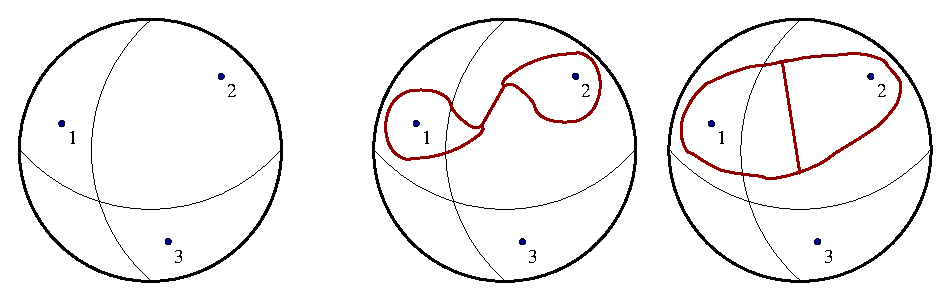
\includegraphics[width=\textwidth]{sfera3}
  \caption{A thrice-punctured sphere and two distinct deformation
    retracts, which are not isomorphic as graphs.}
  \label{fig:sphere-retracts}
\end{figure}
We can refine this correspondence: a theorem proved independently by
J.~A. Jenkins \cite{jenkins;annals} and K.~Strebel
\cite{strebel;quadratic-differentials;1983} provides the key tool: the
construction of fatgraphs from smooth complex curves.

\begin{definition}
  A quadratic differential $q$ on a Riemann surface $S$ is a
  (meromorphic) section of $(T^*S)\tp2$.
\end{definition}
The set of vectors in $T_zS$ on which $q$ takes real non-negative
values forms a real line in $T_zS$: therefore, they make up a
foliation $F = F_qS$ on $S - \{\text{poles of $q$}\}$. The non-compact
leaves of $F$ together with zeroes of $q$ form the ``critical locus''
of~$q$.  Call $F$ the ``horizontal'' foliation associated with $q$.

The set of vectors in $T_zS$ on which $q$ takes a purely imaginary
value form a perpendicular foliation $F^\perp$, whose leaves connect
either two distinct poles $x_i$ and $x_j$, or a pole $x_i$ and a zero
$v_j$.  Call $F^\perp$ the ``vertical'' foliation associated with $q$.

Every quadratic differential $q$ induces a metric (away from the
critical locus) by $\ud s^2 = \abs{q(z)} \cdot \abs{\ud z}$.

\begin{theorem}[Jenkins, Strebel; {\cite[Theorem 23.2 and
    23.5]{strebel;quadratic-differentials;1983}}] 
  \label{thm:JS}
  For any complex analytic curve $S$ with $n$ marked points $x_1, \ldots,
  x_n$, and any assignment of real positive numbers $p_1, \ldots, p_n$,
  there exists one and only one quadratic differential $q$ such that:
  \begin{itemize}
  \item the only poles of $q$ occur at the marked points $x_1, \ldots, x_n$
    with second residue $p_1, ..., p_n$, that is, in a local
    coordinate $z_i$ near $x_i$ we have:
    \begin{equation*}
      q = -(p_i/2\pi)^2 \cdot \d z_i^2 / z_i^2 + \text{higher order terms};
    \end{equation*}
  \item the non-critical real trajectories of $F_q$ are simple closed
    circles around $x_i$.
  \end{itemize}
  Furthermore, $q$ has the following properties:
  \begin{itemize}
  \item every nonsingular closed leaf circling around $x_i$ has length
    $p_i$ in the flat metric induced by $q$.
  \item the critical locus of $q$ is a graph $G$ embedded in $S$;
  \item the complement $S - G$ of the critical locus is a collection
    of disks $\{D_i | i=1,\ldots,n\}$, each one centered at a pole $x_i$, and
    the projective class of the collection of radii of disks $\{D_i\}$
    equals the projective class $[p_1, \ldots, p_n]$.
  \end{itemize}
\end{theorem}
The critical graph $G$ inherits a structure of embedded fatgraph
with metric from the ambient surface $S$: the length of an edge $\alpha$ is
the one measured in the metric induced by the quadratic differential.
Furthermore, Jenkins-Strebel's theory states that $G$ has a vertex of
valence $k+2$ where $q$ has a zero of order $k$, therefore, vertices
of $G$ have valence $\geq3$. 

Since the markings $x_1, \ldots, x_n$ are \emph{ordered}, $G$ has an
additional structure of \emph{numbered} fatgraph.



\section[Combinatorial moduli space of curves]
  {Combinatorial analogues of the moduli space of smooth curves}
\label{sec:mgn-comb}

We shall now construct (orbi)cell-complex analogues of the Teichm\"uller
space and the moduli space of smooth curves, whose cells are indexed
by fatgraphs.  They will come equipped with a homotopy
equivalence to $\T_{g,n}$ and $\M_{g,n}$.

References to this construction are scattered in the literature, and
there are many variants and quirks; see
\cite{harer;cohomology-of-moduli,%
  harer;cohomological-dimension,%
  kontsevich;intersection-theory;1992,%
  looijenga;cellular-decomposition,%
  penner:math.GT/0210326}.


\subsection{Construction of $\Tcomb_{g,n}$ and $\Mcomb_{g,n}$}
\label{sec:mgn-comb-construction}

Let $G$ be a fatgraph (embedded or abstract) of genus $g$ with $n$
numbered boundary components.  A topological simplex is spanned when
varying the metric data $(\ell_\alpha)_{\alpha \in \Edges{G}}$; gluing
these cells one recovers the whole $\T_{g,n}$ (when using
\emph{embedded} fatgraphs), or $\M_{g,n}$ (when using \emph{abstract}
fatgraphs).  A construction of $\Tcomb_{g,n}$ and $\Mcomb_{g,n}$ can
be found in \cite{penner:math.GT/0210326}, although the procedure
outlined here extends the construction of $\Mcomb_{g,n}$ given in
\cite{kontsevich;intersection-theory;1992}.

Call a set $X \subseteq \Edges{G}$ negligible whenever it is \emph{not} the
support of a non-trivial homological cycle.  For an abstract ribbon
graph $G$, define a topological simplex $\Delta(G)$:
\begin{equation*}
  \label{eq:rg-cells-moduli}
  \Delta(G) := \{ \ell: \Edges{G} \to \setR_{\geq0} \,|\,
  {\textstyle \sum}_{\alpha\in\Edges{G}} \ell_\alpha=1 
  \text{ and the zero set of $\ell$ is negligible} \}.
\end{equation*}
It is a contravariant functor from the category of abstract ribbon
graphs to the category of topological spaces: if $G'$ is obtained from
$G$ by contracting the edge $\alpha$, then
\begin{equation}\label{eq:embedding-cells}
  \Delta(G') = \{ \ell \in \Delta(G) | \ell_\alpha = 0 \}.
\end{equation}
By composing with the (covariant) forgetful functor $[G, \iota, \psi_*] \mapsto G$
from embedded fatgraphs to abstract fatgraphs, we define a
contravariant functor $T: \ERG_{g,n} \mapsto \category{Top}$ from the
category of embedded fatgraphs to the category of topological
spaces.
\begin{equation*}
  \label{eq:rg-cells-teichmueller}
  T[G, \iota, \psi_*] := \Delta(G).
\end{equation*}

The category $\ERG$ forms an inverse system over the set of its
objects, by stipulating that $G' > G$ iff $G'$ is obtained from $G$ by
(a sequence of) contraction of edges.  Therefore, the image $T\ERG$ is
a direct system in $\category{Top}$, and we can form its direct limit.
\begin{definition}
  The combinatorial Teichm\"uller space is the limit of the direct
  system $T\ERG_{g,n}$:
  \begin{equation*}
    \Tcomb_{g,n} := \varinjlim T[G, \iota, \psi_*],
  \end{equation*}
  where $[G, \iota, \psi_*]$ ranges in the category $\ERG_{g,n}$ of embedded
  fatgraphs of genus $g$ with $n$ numbered boundary components.
\end{definition}
$\Tcomb_{g,n}$ is obtained by gluing topological simplices $\Delta(G)$ alongside
the boundary: if $[G', \iota', \psi'_*]$ is obtained from $[G, \iota, \psi_*]$ by
contraction of an edge $\alpha$, then $\Delta(G')$ is identified with the face
of $\Delta(G)$ where $\ell_\alpha = 0$ by formula~\ref{eq:embedding-cells}.

Points of the topological space $\Tcomb_{g,n}$ are (equivalence
classes of) metrized embedded fatgraphs $[G, \iota, \psi_*, \ell]$, where $\ell
\in T[G, \iota, \psi_*]$; it is easy to check that any $[G, \iota, \psi_*, \ell] \in
\Tcomb_{g,n}$ has a unique representative such that $\ell_\alpha > 0$ for all
$\alpha \in \Edges{G}$.  Perimeter maps $p_\beta: \Tcomb_{g,n} \to \setR_{>0}$ are
well-defined; write $p_j$ for the perimeter of the $j$-th boundary
component.

In a similar fashion, we can construct $\Mcomb_{g,n}$.
\begin{definition}
  The combinatorial moduli space of curves is the direct limit of the
  functor $\Delta$:
  \begin{equation*}
    \Mcomb_{g,n} := \varinjlim \Delta(G),
  \end{equation*}
  where $G$ ranges in the category $\RG_{g,n}$ of abstract ribbon
  graphs of genus $g$ with $n$ numbered boundary components.
\end{definition}

\subsubsection{Kontsevich' compactification of $\Mcomb_{g,n}$}
\label{sec:mbarcomb}
The construction of $\Mcomb_{g,n}$ can be done with slightly changed
rules: if we define a set $X \subseteq \Edges{G}$ to be negligible iff it does
not contain \emph{all} edges bounding a hole, then we can define a
contrafunctor $\overline{M}(G)$ and a topological space:
\begin{equation*}
  \label{eq:kontsevich-4}
  \Mbarcomb_{g,n} := \varinjlim \overline{M}(G).
\end{equation*}
$\Mbarcomb_{g,n}$ turns out to be a compactification of the orbifold
$\Mcomb_{g,n}$, and a quotient of the Deligne-Mumford compactification
$\Mbar_{g,n} \times \Delta^n$.

\subsubsection{Homotopy equivalence with moduli spaces}
\label{sec:homotopy-equiv}
\begin{theorem}[Harer, Mumford, Thurston;
  \cite{%
    harer;cohomological-dimension,%
    looijenga;cellular-decomposition,%
    penner:math.GT/0210326%
  }]
  \label{thm:HMT}
  The Jenkins-Strebel construction defines homeomorphisms:
  \begin{equation*}
    \T_{g,n} \times \Delta^n \to \Tcomb_{g,n}, 
    \qquad
    \M_{g,n} \times \Delta^n \to \Mcomb_{g,n}, 
    \qquad 
    \Mbar_{g,n} \times \Delta^n \to \Mbarcomb_{g,n}.
  \end{equation*}
\end{theorem}

The reverse maps
\begin{equation*}
  \Tcomb_{g,n} \to \T_{g,n} \times \Delta^n \to \Delta^n,
  \qquad
  \Mcomb_{g,n} \to \M_{g,n} \times \Delta^n \to \Delta^n
\end{equation*}
are the perimeter map $\pi := (p_1, \ldots, p_n)$, where $p_j$ is the
perimeter of the $j$-th boundary component $\beta_j$.  For any given $p^\circ
= (p_1^\circ, \ldots, p_n^\circ) \in \Delta^n$, the fiber $\pi^{-1}(p^\circ)$ is isomorphic
to $\M_{g,n}$ (resp.\ $\T_{g,n}$), thus, $\pi$ induces a triangulation
of $\M_{g,n}$ (resp.\ $\T_{g,n}$).

\subsubsection{Cell structure of $\Mcomb_{g,n}$}
\label{sec:cell-structure}
The functorial action of $\Gamma_{g,n}$ on $\ERG_{g,n}$ induces an action
on $\Tcomb_{g,n}$, which permutes cells $T({\tilde G})$ by PL
isomorphisms.
\begin{lemma}
  \label{lemma:penner-kontsevich-bridge}
  $\Mcomb_{g,n}$ is the quotient space of $\Tcomb_{g,n}$ by the
  cellular action of the mapping class group $\Gamma_{g,n}$.
\end{lemma}
\begin{proof}
  If $G \in \RG_{g,n}$ is any abstract fatgraph, then map $\Delta(G)$ into
  $\Tcomb_{g,n} / \Gamma_{g,n}$ by the following procedure: pick any representative
  embedding ${\tilde G} = [G, \iota, \psi_*] \in \ERG_{g,n}$ of $G$ and compose
  the isomorphism $\Delta(G) \cong T(\tilde G)$ with the quotient projection
  $T(\tilde G) \to \Tcomb_{g,n}/\Gamma_{g,n}$.  The mapping is well-defined:
  if $[G, \iota, \psi_*]$ and $[G, \iota', \psi'_*]$ are two distinct embeddedings
  of $G$, then ${\tilde \iota}, {\tilde \iota'}: S(G) \to S$ are homemorphisms,
  and, for any $\ell \in \Delta(G)$, ${\tilde \iota'} \circ {\tilde \iota}^{-1}$ is
  differentiable with respect to the analytic structure $S(G, \ell)$.
  Therefore, if $\phi := ({\tilde \iota}')^{-1} \circ {\tilde \iota}$, then $[G, \iota,
  \psi_*] = \phi \cdot [G, \iota', \psi'_*]$.

  By definition of direct limit, a map $\Phi: \Mcomb_{g,n} \to
  \Tcomb_{g,n} / \Gamma_{g,n}$ is induced.  It is surjective: every point in $\Tcomb /
  \Gamma$ is a projection of a point $[G, \iota, \psi_*] \in \Tcomb$, therefore it
  is in the image of $G \in \Mcomb$.  Moreover, $\Phi$ is injective: if $G$ and $G'$
  map to the same point in $\Tcomb / \Gamma$, then there is some $\phi \in \Gamma$
  such that $[G, \iota, \psi_*] = \phi \cdot [G', \iota', \psi'_*] = [G', \phi \circ \iota, \psi'_* \circ
  \phi]$; therefore, there is $\phi' \in \Diff^0$ such that $\phi' \circ \iota = \phi \circ \iota'$.
  Thus $f = \iota' \circ \iota^{-1}: G' \to G$ is a isomorphism of ribbon
  graphs.
\end{proof}

\begin{lemma}
  \label{lemma:isotropy}
  The isotropy group $\Gamma_{{\tilde G}}$ of the cell $T{\tilde G} \hookrightarrow
  \Tcomb_{g,n}$ is (isomorphic to) the automorphism group $\Aut G$ of
  the abstract fatgraph $G$ underlying ${\tilde G}$.
\end{lemma}
\begin{proof}
  If $a \in \Aut G$, then $S(a, \ell)$ is an automorphism of $S(G, \ell)$ for
  any metric $\ell$.  If $\ell \in \Delta(G)$ varies continuously, then so does
  $S(a, \ell)$.  Therefore, an element of $\Gamma_{{\tilde G}} \subseteq \Gamma_{g,n}$ is defined.

  Conversely, let $\tau \in \Gamma_{g,n}$ fix the cell $T{\tilde G}$
  \emph{setwise}.  If $q$ is the Jenkins-Strebel quadratic
  differential inducing the complex analytic structure corresponding
  to the metric $\ell \in T({\tilde G})$, then $\tau^*q$ defines a quadratic
  differential corresponding to a point in $T{\tilde G}$, so it has
  critical graph ${\tilde G}$.  But, since $q$ has critical graph
  ${\tilde G}$, $\tau^*q$ has critical graph $\tau({\tilde G})$. Therefore,
  $\tau$ restricts to a fatgraph isomorphism, so a map $\Gamma_{{\tilde
      G}} \to \Aut G$ is defined.
\end{proof}
Let $M(G)$ be the image in $\Mcomb_{g,n}$ of a simplex $T({\tilde G})$,
where ${\tilde G}$ is an embedding of $G$.  By \ref{lemma:isotropy},
the image $M(G)$ is the quotient of $\Delta(G)$ by $\Aut G$; therefore,
$\Mcomb_{g,n}$ is a orbifold.\FIXME{%
  Questo non basta per definire un'orbifold: occorre anche dimostrare
  una relazione tra $\Aut G$ e $\Aut G'$, quando $G'$ \`e una faccia di
  $G$.}
The action of $\Gamma_{g,n}$ commutes with the face operators, so
$M(G)$ is a face of $M(G')$ iff $G'$ is obtained from $G$ by
contraction of a non-loop edge.

Cells $T({\tilde G})$ and $M(G)$ have real dimension
$\card{\Edges{G}}$; therefore, simplices of maximal dimension are
labeled by graphs with all vertices of valence $3$ (see
\eqref{eq:10}). The union of these cells is a dense subset of
$\Tcomb_{g,n}$ (resp.~$\Mcomb_{g,n}$) with non-void interior.



\section{The fatgraph complex}
\label{sec:ribbon-graph-complex}

Harer \cite{harer;cohomological-dimension}, introduced a simplicial
complex related to the Teichm\"uller space $\T_{g,n}$, which, when
recast in terms of fatgraphs, provides the needed link between the
fatgraph complex and (co)homology of $\M_{g,n}$.  


\subsection{Arc-systems}
\label{sec:arc-systems}

\begin{definition}
  An arc-system $[u_1, \ldots, u_k]$ of rank $k$ is an isotopy class
  rel~$\{x_1, \ldots, x_n\}$ of $k$ properly imbedded arcs $u_i : [0,1] \to S$
  such that:
  \begin{itemize}
  \item every $u_i$ has its endpoints in the set $\{x_1, \ldots, x_n\}$;
  \item if $i \neq j$, then $u_i$ meet $u_j$ at endpoints only, if at all;
  \item no $u_i$ is null-homotopic rel~$\{x_1, \ldots, x_n\}$;
  \item no $u_i$ is homotopic rel~$\{x_1, \ldots, x_n\}$ to $u_j$, for $i \neq
    j$;
  \end{itemize}
  An arc-system $[u_1, \ldots, u_k]$ is said to \emph{fill up} the curve
  $S$ iff all connected components of $S - \bigcup\{u_i\} - \{x_1,\ldots x_n\}$ are
  either disks or once-punctured disks.
\end{definition}
Note that a connected component of the complement of a filling
arc-system can only be punctured at a marked point $x_i$.

Arc-systems may be organized into a semi-simplicial complex.
\begin{definition}
  $X$ is the semi-simplicial complex having a simplex $\langle u_1, \ldots, u_k\rangle$
  for every rank $k$ arc-system $[u_1, \ldots u_k]$, with the proviso that
  $\langle u'_1, \ldots, u'_l\rangle$ is a face of $\langle u_1, \ldots, u_k\rangle$ iff $\{ [u'_1], \ldots,
  [u'_l] \} \subset \{ [u_1], \ldots, [u_k] \}$.
  
  $X_\infty$ is the subcomplex of all those simplices $\langle u_1, \ldots, u_k\rangle$
  that do not fill up the surface $S$.
\end{definition}
By definition of $X_\infty$, any simplex in $X$ whose vertices are a subset
of the vertices of $\sigma_\bullet \in X_\infty$ is itself a simplex in $X_\infty$.

There is a natural action of $\tau \in \Gamma_{g,n}$ on $X$ given by $\tau \cdot [u_1, \ldots
u_k] := [\tau \circ u_1, \ldots, \tau \circ u_k]$; it preserves $X_\infty$, so it restricts to
an action on $X - X_\infty$.

If $K$ is any semi-simplicial complex, denote by $|K|$ its geometric
realization.  Let $\Delta^n$ be the $n$-dimensional geometric
simplex $\{ b_* \in \setR^{n+1} | b_0 + \cdots + b_n = 1 \}$.
\begin{theorem}[Harer, {\cite[Theorem
    1.3]{harer;cohomological-dimension}}]
  \label{thm:H}
  There exists a $\Gamma_{g,n}$-equivariant homeomorphism $\Phi: \T_{g,n} \times
  \Delta^n \to |X - X_\infty|$.
\end{theorem}
This is infact another application of Theorem~\ref{thm:JS}.  We only sketch
part of the proof here in order to highlight the features needed in the
sequel. 

Given a marked complex analytic curve $S$ and barycentric coordinates
$b_0 + \cdots + b_n = 1$, by Jenkins-Strebel's Theorem~\ref{thm:JS} there is a
quadratic differential $q$ that has poles at the marked points $\{ x_1,
\ldots, x_n \}$ such that its second residue at $x_i$ is $b_i$.

Form the horizontal and vertical foliations $F$, $F^\perp$ induced by $q$,
as in \ref{sec:strebel}.  Leaves of $F^\perp$ either connect a marked
point $x_i$ (a pole of $q$) to another pole or to a zero point of $q$.
Let $F^\perp_0$ be the collection of leaves of $F^\perp$ that join poles of
$q$; it breaks up into parallel families, where two leaves are
parallel iff they are connected by a homotopy in $S$ fixing the zeroes
and the poles of $q$.  Select one leaf $u_j$ from each family, and
form an arc-system $U = [u_1, \ldots, u_k]$.

Let $G$ be the critical graph of $q$.  Each edge $\alpha \in \Edges{G}$ meets
only \emph{one} arc $u_i$, and they intersect transversally and at one
point only.  Therefore we can associate with every arc $u_i$ the
$q$-length $\ell_i$ of the unique edge $\alpha$ intersecting $u_i$.  

Let $\Phi(S, b_*)$ be the point in the geometric simplex $|\langle u_1, \ldots
u_k\rangle|$ corresponding to the projective class $[\ell_1:\cdots:\ell_k]$.  This
defines a map $\Phi$ from $\T_{g,n} \times \Delta^n$ to $|X - X_\infty|$, which is
proven to be a homeomorphism \cite{harer;cohomological-dimension,
  looijenga;cellular-decomposition}.

\begin{remark}
  \label{rem:approaching-face}
  When the length $\ell_j$ approaches $0$, the point $\Phi(S, b_*)$
  approaches a point on a face of the simplex $|\langle u_1, \ldots,
  u_j, \ldots, u_k\rangle|$; this face is identified with the simplex
  $|\langle u_1, \ldots, \widehat{u_j}, \ldots, u_k\rangle|$.
\end{remark}


\subsection{From arc-systems to fatgraphs}
\label{sec:arcs-to-rg}

Given a graph $U$ drawn on a Riemann surface $S$, recall that the dual
graph $G$ is a graph having a vertex for every connected component of
$S - u$, and an edge for every edge of $U$.  Corresponding edges of
graphs in a duality pair meet at a single point, and we may assume
that they cross transversely.
\begin{lemma}
  \label{lemma:arcs-to-rg}
  There's an equivariant bijective correspondence between arc-systems
  $U \in X - X_\infty$ and embedded fatgraphs ${\tilde G} \in \ERG_{g,n}$,
  the graph corresponding to an arc-system $U$ being the dual graph to
  $U$ in the ambient surface.
\end{lemma}
\begin{proof}
  Let $U = [u_1, \ldots, u_k] \in X - X_\infty$ be an arc-system on the Riemann
  surface $S_{g,n}$.  Any choice of barycentric coordinates $b_0 + \cdots +
  b_k = 1$ identifies a point in the associated geometric
  symplex $|U| \subseteq |X - X_\infty|$; by the proof of Harer's Theorem~\ref{thm:H}
  this corresponds to a complex analytic structure on $S_{g,n}$ (a
  point in $\T_{g,n} \times \Delta^n$) determined by a quadratic differential $q
  = q(u, b_*)$, such that each arc $u_i$ is a regular curve in the
  vertical foliation $F^\perp$ associated to $q$.  Let ${\tilde G}$ be the
  critical graph of $q$; it is endowed with a structure of
  \emph{embedded} fatgraph.  By construction, ${\tilde G}$ is the
  dual graph of $U$.

  Conversely, suppose initially that $G$ has no loops.  Let ${\tilde
    G}$ be a fatgraph embedded in the surface $S = S(G)$.  Break up
  $S$ into closed triangles $\{ T_\alpha \}$ as in
  Lemma~\ref{lemma:S-functor}(b).  Form the dual graph to ${\tilde G}$:
  for each $\{ T_{\alpha^\pm} \}$, let $u_\alpha^\pm$ be the arc
  connecting the midpoint of $\alpha \in \Edges{{\tilde G}}$ to the
  vertex of $T_{\alpha^\pm}$ opposite to $\alpha$, and let $u_\alpha$
  be the arc obtained by joining $u_\alpha^\pm$ at their common
  endpoint.  Then $U = [u_{\alpha_1}, \ldots, u_{\alpha_k}]$ is a
  filling arc-system: indeed, each connected component of $S - U$ is
  homeomorphic to one of the open sets $V_\gamma$ (with $\gamma \in
  \Vertices{G}$), therefore it is a disk.
  If $G$ has any loops, the same construction can be repeated, but
  only one of the two halves $\lambda'$, $\lambda''$ of a loop
  $\lambda$ should be  considered for defining the arc $u_\lambda$.

  This correspondence is equivariant: if $\tau \in \Gamma_{g,n}$ then point
  $b_*$ in $|\tau u|$ corresponds to analytic structure induced by the
  differential $\tau^*q$, which has $\tau({\tilde G})$ as critical graph.
  On the other hand, $\tau({\tilde G})$ has dual graph $\tau u$.
\end{proof}

Note that, if an order of the vertices of the simplex $|U|$ is given,
then an order of the edges of ${\tilde G}$ is induced.

\begin{lemma}
  \label{lemma:erg-loop}
  Embedded fatgraphs with a loop correspond to arc-system simplices
  in $X$ with a face on $X_\infty$: every loop in a fatgraph ${\tilde G}$
  corresponds to a face on $X_\infty$ in the dual arc-system.
\end{lemma}
\begin{proof}
  Let ${\tilde G}$ be an embedded fatgraph.  If no edge of
  ${\tilde G}$ is a loop, then any contraction of an edge in ${\tilde
    G}$ produces an embedded fatgraph in $\ERG_{g,n}$, which again
  corresponds to a simplex in $X - X_\infty$.  Therefore, embedded ribbon
  graphs with no loops identify cells in $X$ with no face on $X_\infty$.

  Now let ${\tilde G}$ be an embedded fatgraph having a loop $\lambda \in
  \Edges{G}$, and let $U = \langle u_1, \ldots, u_k\rangle$ be the arc-system simplex
  corresponding to ${\tilde G}$ according to Lemma~\ref{lemma:arcs-to-rg}.
  Contraction of $\lambda$ in ${\tilde G}$ is not admissible, as it would
  change the genus and/or the puncture number of ${\tilde G}$;
  correspondingly, if $U'$ is the face of $U$ obtained by omitting the
  unique arc that intersects $\lambda$, then $U'$ does not fill up the
  ambient surface: two marked points fall in the same connected
  component of $S - U'$.
\end{proof}

\begin{lemma}
  \label{lemma:PL-face}
  There is a canonical PL isomorphism between $|U|$ and
  $T({\tilde G}) = \Delta(G)$.

  This correspondence is compatible with the face operations: if $U' \in
  X - X_\infty$ is a face of $U \in X - X_\infty$, then the dual graph ${\tilde
    G}'$ is obtained from ${\tilde G}$ by contraction of a non-loop
  edge, and the PL isomorphism $|U| \isoarrow T({\tilde G})$ restricts
  to $|U'| \isoarrow T({\tilde G}')$ on the faces.
\end{lemma}
By Lemma~\ref{lemma:PL-face}, the face operators on the two set of
simplices are compatible with this PL isomorphism, so we can glue
isomorphisms $|\langle u_*\rangle| \to |G|$ to form a PL isomorphism $|X - X_\infty| \to
\Tcomb_{g,n}$.
\begin{proof}
  The canonical isomorphism is a direct consequence of the bijective
  correspondence of edges of ${\tilde G}$ with arcs of $U$: the
  coordinate $b_i$ in $|U|$ corresponding to the arc $u_i$ is sent to
  the coordinate $\ell_i$ on the unique edge $\alpha_i$ meeting $u_i$.  This
  assignment is compatible with the face operators: $b_i=0$ identifies
  points on the face $|u_1, \ldots, \widehat{u_i}, \ldots, u_k|$ of $|U|$, and
  $\ell_i = 0$ identifies the face of $\Delta(G)$ corresponding to the graph
  $G/\alpha_i$ where the non-loop edge $\alpha_i$ has been contracted to a point.
\end{proof}


\subsection{Equivariant homology of $\T_{g,n}$ and the complex of
  fatgraphs}
\label{sec:rg-complex}

\begin{definition}\label{dfn:orientation}
  An orientation of a fatgraph $G$ is an orientation of the vector
  space $\setQ\Edges{G}$, that is, the choice of an order of the edges of
  $G$, up to even permutations.
\end{definition}
Giving an orientation on $G$ (resp.~${\tilde G}$) is the same as
orienting the simplex $\Delta(G)$ (resp.~$T({\tilde G})$).

If $G$ is a fatgraph with $p$ edges, let $W_G := \bigwedge^p \setQ\Edges{G}$
be the 1-dimensional vector space generated by wedge products $\alpha_1 \land \ldots
\land \alpha_p$ of edges of $G$.  Every $f \in \Aut G$ induces a map $f:
\Edges{G} \to \Edges{G}$ on the edges and thus a map $f_*: \alpha_1 \land \ldots
\land \alpha_p \mapsto f(\alpha_1) \land \ldots \land f(\alpha_p)$.  Trivially, $f_*(\alpha_1 \land
\ldots \land \alpha_p) = \pm \alpha_1 \land \ldots \land \alpha_p$, depending on whether $f$ preserves or
reverses the orientation of $G$.

\begin{definition}\label{dfn:orientable}
  Say that $G$ is \emph{orientable} iff it has no
  orientation-reversing automorphisms.
\end{definition}

Form a differential complex of orientable fatgraphs as follows.
\begin{definition}
  The complex $(W_*, D)$ of orientable fatgraphs is defined by:
  \begin{itemize}
  \item $W_p := \bigoplus_G W_G$, where $G$ runs over orientable fatgraphs
    with $(2g + n - 1 + p)$ edges;
  \item $D: W_p \to W_{p-1}$ is given by $D := \sum_1^p (-1)^i d_i$ where:
    \begin{equation*}
      d_i(\alpha_1 \land \ldots \land \alpha_p) :=
        \alpha_1 \land \ldots \land \widehat{\,\alpha_i\,} \land
        \ldots \land \alpha_p,
    \end{equation*}
    iff $\alpha_i$ is not a loop and $G/\alpha_i$ is orientable, and
    \begin{equation*}
      d_i(\alpha_1 \land \ldots \land \alpha_p) := 0,
  \end{equation*}
  otherwise.
  \end{itemize}
\end{definition}

Call a fatgraph with one vertex only a \emph{clover}; the number $l$
of edges of a clover of genus $g$ is readily computed by
\eqref{eq:euler-characteristics-of-fatgraphs}:
\begin{equation}
  \label{eq:9}
  l_{\min} = 1 - \chi(G) = 2g + n - 1.
\end{equation}
On the other hand, the number of vertices (and edges too) is maximum
in a fatgraph when all vertices are 3-valent; from
\begin{equation*}
  3v = 2l, 
  \qquad
  v - l = \chi(G) = 2 - 2g - n,
\end{equation*}
we reckon:
\begin{equation}
  \label{eq:10}
  l_{\max} = 6g + 3n - 6, 
  \qquad 
  v_{\max} = 4g + 4n - 4
\end{equation}
From equations~\eqref{eq:9} and~\eqref{eq:10} we see that $W_*$ is a
finite complex of length $4g + 2n - 5$, which is already predicted by
result of Harer on the equivariant spine of $\T_{g,n}$
\cite{harer;cohomological-dimension}.

Every oriented fatgraph $(G, \omega)$ defines an element $\omega_G \in W_G$ by
taking the wedge product of edges of $G$ in the order given by $\omega$;
conversely, any $\alpha_1 \land \ldots \land \alpha_p \in W_G$ defines an orientation on $G$ by
setting $\alpha_1 < \ldots < \alpha_p$.

\begin{theorem}\label{thm:fatgraph-homology}
  The $\Gamma_{g,n}$-equivariant homology of $\T_{g,n}$ with rational
  coefficients is computed by the complex of oriented fatgraphs
  $(W_*, D)$, that is, there exists an isomorphism
  \begin{equation*}
    H^{\Gamma_{g,n}}_*(\T_{g,n}, \setQ) \cong H_*(W_*, D)
  \end{equation*}
\end{theorem}
\begin{proof}
  The genus and puncture number will be fixed throughout, so for
  brevity, put $\Gamma := \Gamma_{g,n}$, $\T := \T_{g,n}$ and $\Tcomb :=
  \Tcomb_{g,n}$.  

  By Theorem~\ref{thm:HMT}, we have:
  \begin{equation*}
    H^\Gamma_*(\T, \setQ) = H^\Gamma_*(\Tcomb, \setQ). 
  \end{equation*}
  Recall that $H^\Gamma_*(\Tcomb, \setQ)$ can be defined as the homology of the
  double complex $P_* \otimes C_*(\Tcomb, \setQ)$, where $P_*$ is any projective
  resolution of $\setQ$ over $\setQ[\Gamma]$.  The spectral sequence $E^1_{pq} :=
  H_q(P_* \otimes_\Gamma C_p) = H_q(\Gamma, C_p)$ abuts to $H^\Gamma_{p+q}(\Tcomb)$ (see
  \cite[VII.5 and VII.7]{brown}).

  The space $\Tcomb_{g,n}$ has, by definition, an equivariant
  cellularization with cells indexed by embedded fatgraphs of
  genus $g$ with $n$ numbered boundary components.  Let $R_p$ be a set
  of representatives for the orbits of $p$-cells under the action of
  $\Gamma$.  By Lemma~\ref{lemma:penner-kontsevich-bridge}, $R_p$ is in
  bijective correspondence with the set of abstract fatgraphs
  having $p$ edges, and the orientation of a cell translates directly
  to an orientation of the corresponding graph.  For each geometric
  simplex $T{\tilde G} \subseteq \Tcomb$, let $\Gamma_{\tilde G}$ be its
  isotropy group, and let $\setQ{\tilde G}$ be the $\Gamma_{\tilde
      G}$-module consisting of the $\setQ$-vector space generated by an
  element $\Delta$ on which $\Gamma_{\tilde G}$ acts by the orientation
  character: $\tau \cdot \Delta = \pm \Delta$ depending on whether $\tau$ preserves or
  reverses the orientation of the cell $T{\tilde G}$.  By
  Lemma~\ref{lemma:isotropy}, there is an isomorphism between $\Gamma_{\tilde
      G}$ and $\Aut G$; if $\tau \in \Gamma_{\tilde G}$ reverses
  (resp.~preserves) orientation of $T{\tilde G}$, then the
  corresponding $f \in \Aut G$ reverses (resp.~preserves) orientation on
  $G$.  Therefore, $\setQ{\tilde G}$ and $W_G$ are isomorphic as $\Aut G =
  \Gamma_{T{\tilde G}}$ modules.

  Following \cite[p.~173]{brown}, let us decompose (as a $\Gamma$-module)
  \begin{equation*}
    C_*(\Tcomb, \setQ) = \bigoplus_{G \in R_p} W_G;
  \end{equation*}
  then, by Shapiro's lemma \cite[III.6.2]{brown}, we have:
  \begin{equation*}
    H_q(\Gamma, C_p) \cong \bigoplus_{G \in R_p} H_q(\Gamma_{\tilde G}, \setQ{\tilde G}) \cong
    \bigoplus_{G \in R_p} H_q(\Aut G, W_G). 
  \end{equation*}
  Since $\Aut G$ is finite and we take rational coefficients, then
  $H_q(\Aut G, W_G) = 0$ if $q > 0$ \cite[III.10.2]{brown}.  On the
  other hand,
  \begin{equation*}
    H_0(\Aut G, W_G) =
    \begin{cases}
      0
      &\text{if $G$ has an orientation-reversing automorphism,}
      \\
      W_G
      &\text{if $G$ has \emph{no} orientation-reversing automorphisms%
        \footnote{In other words: $G$ is orientable, so $\Aut G$ acts
          trivially on $W_G$.}}
    \end{cases}
  \end{equation*}
  Let $R'_p$ be the collection of all orientable fatgraphs with
  $p$ edges.  Substituting back into the spectral sequence, we see
  that only one column survives:
  \begin{align}
    \label{eq:11}
    E^1_{p,0} &= \bigoplus_{G \in R'_p} W_G = W_p,
    &
    \\
    \label{eq:12}
    E^1_{p,q} &= 0
    &\text{for all $q > 0$,}
  \end{align}
  That is, $E^1_{pq}$ reduces to the complex $(E^1_{*,0}, d^1)$.

  Finally, we show that the differential $d^1: E^1_{p,0} \to E^1_{p-1,
    0}$ corresponds to the differential $D: W_p \to W_{p-1}$ under the
  isomorphism formula~\ref{eq:11}; this will end the proof.  Indeed, we
  shall prove commutativity of the following diagram at the chain
  level:
  \begin{equation}
    \label{eq:13}
    \xymatrix{%
      P_* \otimes W_p
      &
      \bigoplus_{G \in R'_p} P_* \otimes W_G
      &
      \bigoplus_{G' \in R'_{p-1}} P_* \otimes W_{G'} 
      & 
      P_* \otimes W_{p-1} 
      \\
      & 
      P_* \otimes C_p(\Tcomb, \setQ)
      &
      P_* \otimes C_{p-1}(\Tcomb, \setQ) 
      &
      \ar^{\id_P \otimes D} "1,2";"1,3"
      \ar_{\id_P \otimes \partial} "2,2";"2,3"
      \ar_{\theta_p} "1,2";"2,2"
      \ar^{\theta_{p-1}} "1,3";"2,3"
      \ar@{=} "1,1";"1,2"
      \ar@{=} "1,3";"1,4"
    }
  \end{equation}
  which implies commutativity at the homology level:
  \begin{equation*}
    \xymatrix{%
      \bigoplus_{G \in R'_p} H_0(\Aut G, W_G)
      &
      \bigoplus_{G' \in R'_{p-1}} H_0(\Aut G', W_{G'})
      \\
      H_0(\Gamma, C_p(\Tcomb, \setQ))
      &
      H_0(\Gamma, C_{p-1}(\Tcomb, \setQ))
      \ar^{D} "1,1";"1,2"
      \ar_{d^1 = H_0(\Gamma, \partial)} "2,1";"2,2"
      \ar_{\cong} "1,1";"2,1"
      \ar^{\cong} "1,2";"2,2"
    }
  \end{equation*}
  whence the thesis $E^1_{*,0} \cong (W_*, D)$.

  The vertical maps $\theta_p$, $\theta_{p-1}$ in \eqref{eq:13} are the chain
  isomorphisms underlying the $\Gamma$-module decomposition $C_p(\Tcomb, \setQ)
  \cong \bigoplus_{G \in R_p} W_G$.  Taking the boundary of a cell $T{\tilde G} \subseteq
  \Tcomb$ commutes with the $\Gamma$-action: $\partial T(\tau \cdot {\tilde G}) = \tau \cdot \partial
  T({\tilde G})$.  Furthermore, $T({\tilde G}')$ is a cell in
  $\partial T({\tilde G})$ iff ${\tilde G}'$ is obtained from ${\tilde G}$ by
  contraction of an edge; but ${\tilde G}'$ is a contraction of
  ${\tilde G}$ iff the underlying \emph{abstract} fatgraphs $G'$
  and $G$ stand in the same relation.  Thus, the $\Gamma$-complexes $(C_*,
  \partial)$ and $(W_*, D)$ are isomorphic by $\theta_*$, so \eqref{eq:13}
  commutes, as was to be proved.
\end{proof}



%%% Local Variables: 
%%% mode: latex
%%% TeX-master: "index"
%%% x-symbol-8bits: nil
%%% End: 
